\epigraph{``I've got a bad feeling about this"}{Hans Solo}

\section{Geostrophic Wind}\label{geostrophic_wind}
There are a number of forces that can either change the force or direction of wind. Two of the biggest forces of wind vectors are the pressure gradient force and the Coriolis force.

\subsection{Pressure-Gradient Force}
\begin{definition}
The pressure-gradient force is a force acting on air that is due to pressure differences.
\end{definition}

Horizontal variations in pressure create a tendency for movement from higher to lower pressure. The atmosphere, like all systems in nature, is trying to stay at the lowest energy level possible. Therefore, if there is an area of lower pressure nearby, air will freely move from the high pressure area to the low pressure area in order to equalise this energy gradient. To do this, it will attempt to take the shortest distance possible in order to maximise efficiency, which happens to be perpendicular to the isobars\cite{pressuregrad_def}. This phenomenon is described by equation \ref{pressure_grad}, where $P$ is the pressure-gradient force.

\begin{equation}
    \label{pressure_grad}
    P = - \Vec{\nabla} p
\end{equation}

The negative sign at the beginning of the equation designates that we move from high to low across the pressure gradient. The greater the difference in pressure between the two locations, the greater the pressure gradient. A stronger pressure-gradient force usually correlates to a stronger wind vector. It must be noted that the pressure-gradient force is only one component of the forces acting on the actual wind, though, so, air does not normally flow perpendicular to the isobars\cite{pressure_grad}.

\subsection{Coriolis Force}
\begin{definition}
The Coriolis force is an inertial force that acts on objects that are in motion within a frame of reference that rotates with respect to an inertial frame.
\end{definition}

The Coriolis force ultimately results in the diversion of the wind's direction within the atmosphere due to the Earth's rotation. The Earth is spinning in a prograde direction. The Earth is a elongated spheroid, however, to a reasonable good approximation, it can be considered to be a sphere. Due to this fact, all points on the surface of the Earth are travelling at the same angular velocity. As a consequence, however, a point near the equator must have a higher linear velocity, as it must travel a larger distance than a point near the poles. When an object moves either closer or further from the equator its original momentum is preserved, giving the path a diversion off its original course\cite{corioliseffect_def}. If the wind is travelling in accordance with the pressure-gradient force, the wind will be deflected off its original course by the Coriolis force. It must be noted that there isn't a Coriolis force at the equator, however, it increases with intensity as one approaches the poles. The Coriolis force is described by equation \ref{coriolis_force}.

\begin{equation}
    \label{coriolis_force}
    F = \rho U f
\end{equation}

where $f$ is the Coriolis parameter, and is given by equation \ref{f}.

\begin{equation}
    \label{f}
    f = 2 \Omega \sin{\phi}
\end{equation}

One can therefore deduce that the higher the latitude, the higher the Coriolis force. Also, The Coriolis force only acts on air that is already set into motion. The Coriolis force will not set wind into motion, but will only deflect the direction of wind that is already moving. Therefore, it follows that the faster that air is moving, the stronger it is affected by the Coriolis force\cite{coriolis_effect}.

\subsection{Geostrophic Balance}\label{balance}
\begin{definition}
Geostrophic Balance is an exact balance between the Coriolis force and the pressure-gradient force.
\end{definition}

This balance seldom holds true in nature. This concept, however, will lead to the development of a theoretical wind, known as geostrophic wind. First and foremost, lets introduce the horizontal momentum equations.

\begin{equation}
    \frac{Du}{Dt} = -\frac{1}{\rho}\frac{\partial p}{\partial x} + f v
\end{equation}

\begin{equation}
    \frac{Dv}{Dt} = -\frac{1}{\rho}\frac{\partial p}{\partial y} - f  u
\end{equation}

Assuming geostrophic balance, the system is stationary and the first two equations become:  

\begin{equation}
    u = -\frac{1}{\rho f} \frac{\partial p}{\partial y}
\end{equation}

\begin{equation}
    v = \frac{1}{\rho f} \frac{\partial p}{\partial x}
\end{equation}

This is the geostrophic wind, and as mentioned previously, any spatial derivatives within this equation are replaced by a central difference approximation of the derivatives. Therefore, the above equations are rewritten as follows:

\begin{equation}
    u_g = -\frac{1}{\rho f} \frac{\Delta p}{2 \Delta y}
\end{equation}

\begin{equation}
    v_g = \frac{1}{\rho f} \frac{\Delta p}{2 \Delta x}
\end{equation}

\begin{definition}
Geostrophic Wind is the wind that flows parallel to height contours or isobars resulting from an exact balance between the Coriolis force and the pressure-gradient force.
\end{definition}

For the geostrophic flow concept to work, the wind must not be changing speed (is unaccelerated or the acceleration is almost zero). The question remains whether geostrophic wind is a good approximation for the actual wind. The tendency for wind to be accelerated can be measured at various scales of circulation. Meanwhile, the Coriolis acceleration is only related to the speed of the object and its latitude. Thus, as the flow  approaches geostrophic the smaller the actual acceleration is relative to the Coriolis acceleration\cite{geo_wind}.

\begin{definition}
Rossby Number is the ratio of the total acceleration to the Coriolis acceleration.
\end{definition}

If the Rossby number is small (less than one), the geostrophic wind is a reasonably good approximation for geostrophic wind, neglecting the force of friction in this assumption. From table 3.1, generally the geostrophic wind is a good approximation if it is determined at a synoptic scale\cite{geo_wind}. 

\hfill

\begin{center}
\begin{tabular}{|c|c|c|} 
 \hline
 Scale of Circulation & Rossby Number & Yes / No \\
 \hline
 10,000 km & 0.01 & Yes \\
 \hline
 1,000 km & 0.1 & Yes \\
 \hline
 100 km & 1.0 & Not Really \\
 \hline
 10 km & 3.0 & No \\
 \hline
 1 km & 4.0 & No \\
 \hline
\end{tabular}\par
\bigskip
Table 3.1.: Is geostrophic wind a good approximation for the real wind?
\end{center}

\section{Pressure Thickness}\label{pressure_thickness}
\begin{definition}
Pressure Thickness is the measurement of the distance (in metres) between any two constant pressure surfaces.
\end{definition}

\begin{figure}[H]
    \centering
    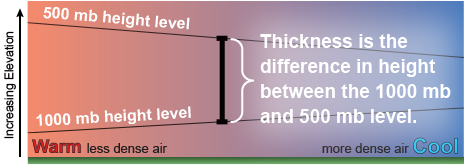
\includegraphics[width=.8\linewidth]{Images/thickness_def.png}
    \caption{Pressure Thickness Definition (provided by the NWS of the USA)}
    \label{thickness_def}
\end{figure}

One of the most common thickness charts used in meteorology is the 1000-500 hPa thickness, and for the purposes of this project, it will be the sole interest. This is the distance between the elevation of the 1,000 hPa and 500 hPa levels. Typically, the 1,000 hPa surface is used to represent sea level but this is just a generalisation. On pressure charts, the last digit (zero) of a thickness value is typically truncated. So, a 1000-500 thickness value of 570 means the distance between the two surfaces is 5,700 metres. The 1000-500 hPa thickness value of 540 is traditionally used to determine rain versus snow. If precipitation is predicted poleward of this 540-thickness line (if the thickness value is less than 540), it is expected that it will be snow. If precipitation is predicted on the equator side of this line (if the thickness value is greater than 540), then it is expected that the precipitation will be in a liquid form. The reason one is able to make such an expectation is due to the fact that the 540-thickness line closely follows the surface freezing temperature of 273 K\cite{thickness}.

\begin{figure}[H]
    \centering
    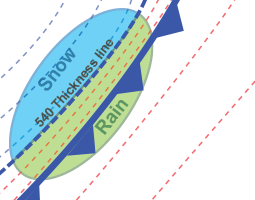
\includegraphics[width=.4\linewidth]{Images/rainsnow_line.png}
    \caption{Rain/Snow Line (provided by the NWS of the USA)}
    \label{rainsnow_line}
\end{figure}

Traditionally, one would determine the pressure thickness between two constant pressure surfaces by utilising the Hypsometric equation, as shown in equation \ref{hypsometric}. For the purposes of this project, and simplicity, the pressure thickness will be determined by using nonlinear regression. 

\begin{definition}
The hypsometric equation relates an atmospheric pressure ratio to the equivalent thickness of an atmospheric layer considering the layer mean of virtual temperature, gravity, and occasionally wind. It is derived from the hydrostatic equation and the ideal gas law.
\end{definition}

\begin{equation}
    \label{hypsometric}
    h = \frac{R \bar{T_v}}{g} \ln{\frac{p_1}{p_2}}
\end{equation}

\begin{definition}
Nonlinear regression is a form of regression analysis in which observational data are modelled by a function which is a nonlinear combination of the model parameters and depends on one or more independent variables.
\end{definition}

In general, there is no closed-form expression for the best-fitting parameters, as there is in linear regression. Usually numerical optimisation algorithms are applied to determine the best-fitting parameters\cite{nonlingress_def}. In the software, the SciPy method, scipy.optimize.curve\_fit, is utilised to perform the nonlinear regression. This method uses nonlinear least squares to fit a function to the data. The algorithm used by this particular method of SciPy is the Levenberg-Marquardt algorithm\cite{scipy_nonlingress}. Following which, the inverse of this modelled function is used to determine the altitude at which the constant pressure surfaces of 1000 hPa and 500 hPa would be.

\begin{definition}
Levenberg-Marquardt algorithm is used to solve non-linear least squares problems. These minimisation problems arise especially in least squares curve fitting.
\end{definition}

As previously mentioned in chapter \ref{2}, atmospheric pressure decreases exponentially with altitude. Therefore, the relationship between atmospheric pressure and altitude, with altitude being the independent variable and atmosphere pressure being the dependent variable, is modelled on an exponential function. The particular exponential function of choice is shown in equation \ref{exponential_function}.

\begin{equation}
    \label{exponential_function}
    a - \frac{b}{c} (1 - \exp(-c x))
\end{equation}

While it is not possible to state the values of $a$, $b$, and $c$ due to the fact they are calculated on a case by case basis, at a given latitude and longitude, the `guess' value of $a$ is 1000, of $b$ is 0.12, and of $c$ is 0.00010. It is also important to note that the mean $R^2$ is approximately 0.99.

\section{Precipitable Water}
\begin{definition}
Precipitable Water is the total atmospheric water vapour contained in a vertical column of unit cross-sectional area extending between any two specified pressure levels.
\end{definition}

Based on the definition, precipitable water can be described mathematically as being:

\begin{equation}
    \label{pwv_1}
    W = \int_{0}^{z} \rho_v dz
\end{equation}

where $\rho_v$ is the density of water vapour, and where $\rho_v$ is defined as:

\begin{equation}
    \rho_v = \frac{\texttt{mass of vapour}}{\texttt{unit volume}}
\end{equation}

Following which, the hydrostatic equation can be applied to equation \ref{pwv_1} in order to replace $dz$ with $dp$. The reason for doing this is that atmospheric pressure is extremely easier to measure, with devices such as weather balloons being readily available.

\begin{equation}
    \label{pwv_derive}
    W = -\int_{p_1}^{p_2} \frac{\rho_v}{\rho g} dp
\end{equation}

Where $p_1$ and $p_2$ are constant pressure surfaces, and where $p_1 > p_2$. Substituting in the definition of density, $\rho_v = \frac{m_v}{V}; \rho = \frac{m_{air}}{V}$, into equation \ref{pwv_derive} results in:

\begin{equation}
    W = -\int_{p_1}^{p_2} \frac{1}{g} \frac{m_v V}{m_{air} V} dp
\end{equation}

\begin{equation}
    \Rightarrow W = - \frac{1}{g} \int_{p_1}^{p_2} \frac{m_v}{m_{air}} dp
\end{equation}

The integration term in this particular equation is the definition for the specific humidity, with the units of measurement being $\frac{kg}{kg}$. The specific humidity can be approximated by the mixing ratio, with an error typically around 4 \%\cite{pwv_def}.

\begin{definition}
Mixing Ratio is the ratio of the mass of a variable atmospheric constituent to the mass of dry air.
\end{definition}

\begin{equation}
    \label{pwv_derive_fin}
    \therefore W = -\frac{1}{g} \int_{p_1}^{p_2} m dp
\end{equation}

The units as given by the equation are $\frac{kg}{m^2}$ (dimensionless), but, the preferred unit of measurement for rainfall is $mm$. The conversion between the two units of measurements is one to one ($1 \frac{kg}{m^2} = 1 mm$) In actual rainstorms, particularly thunderstorms, amounts of rain very often exceed the total precipitable water of the overlying atmosphere. This results from the action of convergence that brings into the rainstorm the water vapour from a surrounding area that is often quite large. Nevertheless, there is general correlation between precipitation amounts in given storms and the precipitable water of the air masses involved in those storms\cite{problems_with_pwv}.

For the purposes of numerically calculating the precipitable water for a given column of air, equation \ref{pwv_derive_fin} is commonly rewritten as the following:

\begin{equation}
    \label{pwv}
    W = -\frac{1}{\rho g} \int_{p_1}^{p_2} \frac{0.622 e}{p - e} dp
\end{equation}

\begin{definition}
Vapour Pressure is the pressure exerted by a vapour when the vapour is in equilibrium with the liquid or solid form, or both, of the same substance. In meteorology, vapour pressure is used almost exclusively to denote the partial pressure of water vapour in the atmosphere.
\end{definition}

For the purposes of this project, the saturated vapour pressure will be utilised, in place of the actual vapour pressure. Saturated vapour pressure is the maximum pressure possible by water vapour at a given temperature. One can determine the saturated vapour pressure using the following equation\cite{balton}:

\begin{equation}
    e = 6.112 \exp(\frac{17.67 T}{T + 243.5})
\end{equation}

Saturated precipitable water on a synoptic scale is a pretty good approximation for the actual precipitable water. In wet periods, the precipitable water is particularly close to the saturated precipitable water. In situations when the precipitable water is close to the saturated precipitable water, the precipitable water changes very little over the day. Saturated precipitable water also makes calculations a whole lot simpler, as specific humidity data is rather difficult to come by. In the release candidate version of the software, a move away from saturated vapour pressure will be made\cite{pwv_error}.

In regards to the numerical calculation of the saturated precipitable water, the SciPy method, scipy.integrate.quad, is utilised in order to determine the definite integral in equation \ref{pwv}. This method integrates the function using a technique from the Fortran library, QUADPACK\cite{scipy_integrate}. 

\section{Primitive Equations}
\begin{definition}
The Primitive Equations, or sometimes known as the Forecast Equations, are a set of nonlinear partial differential equations which approximate global atmospheric circulation, and are utilised in most atmospheric models. 
\end{definition}

These equation are time dependent, and are used to predict the future state of the atmosphere. There are a total of five distinct equations: two of these are for the horizontal wind components, and there is one each for temperature, pressure thickness and precipitable water\cite{nws}. These prediction equations can be written as follows: 

\begin{equation}
    \frac{\partial u}{\partial t} = \eta v - \frac{\partial \Phi}{\partial x} - c_{p} \theta \frac{\partial \Pi}{\partial x} - z \frac{\partial u}{\partial \sigma} - \frac{\partial (\frac{u^2 + v^2}{2})}{\partial x}
    \label{prim_u}
\end{equation}

\begin{equation}
    \frac{\partial v}{\partial t} = - \eta \frac{u}{v} - \frac{\partial \Phi}{\partial y} - c_{p} \theta \frac{\partial \Pi}{\partial y} - z \frac{\partial v}{\partial \sigma} - \frac{\partial (\frac{u^2 + v^2}{2})}{\partial y}
    \label{prim_v}
\end{equation}

\begin{equation}
    \frac{\partial T}{\partial t} = \Vec{v} \cdot \nabla T
    \label{og_primtemp}
\end{equation}

\begin{equation}
    \frac{\partial W}{\partial t} = \Vec{v} \cdot \nabla W
    \label{og_primw}
\end{equation}

\begin{equation}
    \frac{\partial}{\partial t} \frac{\partial p}{\partial \sigma} = u \frac{\partial}{\partial x} \left( x \frac{\partial p}{\partial \sigma} \right) + v \frac{\partial}{\partial y} \left( y \frac{\partial p}{\partial \sigma} \right) + w \frac{\partial}{\partial z} \left( z \frac{\partial p}{\partial \sigma} \right)
    \label{prim_h}
\end{equation}

For the purposes of this project, only equations \ref{og_primtemp} and \ref{og_primw} will be utilised from the above equations. The reason for not utilising equations \ref{prim_u} and \ref{prim_v} is quite simple. Due to utilisation of geostrophic wind, there is an exact balance between the Coriolis force and the pressure gradient force. This implies that there is no acceleration in the geostrophic wind (it doesn't change with time), or described mathematically:

\begin{equation}
    \frac{\partial u}{\partial t}, \frac{\partial v}{\partial t} = 0
    \label{bal_eq}
\end{equation}

This, therefore, makes equations \ref{prim_u} and \ref{prim_v} redundant. Assuming that equation \ref{bal_eq} is true also greatly simplifies the remainder of the equations, as the $\Vec{v}$ component is now constant. The reason for not utilising equation \ref{prim_h} is not as simple. Instead of using this particular equation to calculate the pressure thickness, the mass continuity equation will be utilised in order to forecast the atmospheric density. After which, the Ideal Gas Law (section \ref{ideal}) will be invoked in order to determine the atmospheric pressure; with the pressure thickness between 1000 hPa and 500 hPa being determined in a similar manner to that described in section \ref{pressure_thickness}.  

\subsection{Temperature and Precipitable Water}\label{temp_pwv_section}
To begin, the temperature equation will be the primary focus and was written in equation \ref{og_primtemp} as follows:

\begin{equation}
    \frac{\partial T}{\partial t} = \Vec{v} \cdot \nabla T
\end{equation}

First and foremost, the del operator ($\nabla$) will be expanded into its components as shown in equation \ref{del_operator}. The reason for doing so is that it makes the equation easier to work with down the line.

\begin{equation}
    \Rightarrow \frac{\partial T}{\partial t} = \begin{bmatrix} \Vec{v}_x \\ \Vec{v}_y \\ \Vec{v}_z \end{bmatrix} \cdot \begin{bmatrix} \frac{\partial}{\partial x} \hat{i} \\ \frac{\partial}{\partial y} \hat{j} \\ \frac{\partial}{\partial z} \hat{k} \end{bmatrix} T
    \label{del_operator}
\end{equation}

Taking the dot product results in the following:

\begin{equation}
     \frac{\partial T}{\partial t} = (\Vec{v_{x}} \frac{\partial}{\partial x} \hat{i} + \Vec{v_{y}} \frac{\partial}{\partial y} \hat{j} + \Vec{v_{z}} \frac{\partial}{\partial z} \hat{k}) T
\end{equation}

Expanding the brackets results in:

\begin{equation}
     \frac{\partial T}{\partial t} = \Vec{v_{x}} \frac{\partial T_{x}}{\partial x} + \Vec{v_{y}} \frac{\partial T_{y}}{\partial y} + \Vec{v_{z}} \frac{\partial T_{z}}{\partial z} 
\end{equation}

\begin{equation}
    \Rightarrow \frac{\partial T}{\partial t} = u \frac{\partial T}{\partial x} + v \frac{\partial T}{\partial y} + w \frac{\partial T}{\partial z}
    \label{analytic_temp_final}
\end{equation}

The terms on the RHS are due to advection within the atmosphere.

\begin{definition}
Advection is the transport of a substance or quantity by bulk motion.
\end{definition}

Each $T$ is actually different and related to its respective plane. This is divided by the distance between grid points to get the change in temperature with the change in distance. When multiplied by the wind velocity on that plane, the units $K m^{-1}$ and $m s^{-1}$ give $K s^{-1}$. The sum of all the changes in temperature due to motions in the $x$, $y$, and $z$ directions give the total change in temperature with time\cite{primitive_equations}.

It is not possible to solve this equation analytically, however, one can get an approximate numerical solution by using the finite difference method. To do this, it is necessary to discretize this equation in both space and time, using the central difference scheme. The primary reason for choosing the central difference scheme is that its convergence rate is faster than some other finite difference methods, such as forward and backward differencing. Therefore, discretizing equation \ref{analytic_temp_final} results in:

\begin{equation}
    \frac{T^{n + 1}_{x, y, z} - T^{n - 1}_{x, y, z}}{2 \Delta t} = u \frac{T^{n}_{x+1, y, z} - T^{n}_{x-1, y, z}}{2 \Delta x} + v \frac{T^{n}_{x, y+1, z} - T^{n}_{x, y-1, z}}{2 \Delta y} + w \frac{T^{n}_{x, y, z+1} - T^{n}_{x, y, z-1}}{2 \Delta z}
\end{equation}

The vertical advection term is equal to zero, as there isn't a vertical geostophic wind ($w = 0$):

\begin{equation}
    \frac{T^{n + 1}_{x, y, z} - T^{n - 1}_{x, y, z}}{2 \Delta t} = u \frac{T^{n}_{x+1, y, z} - T^{n}_{x-1, y, z}}{2 \Delta x} + v \frac{T^{n}_{x, y+1, z} - T^{n}_{x, y-1, z}}{2 \Delta y} + \cancelto{0}{w \frac{T^{n}_{x, y, z+1} - T^{n}_{x, y, z-1}}{2 \Delta z}}
\end{equation}

Multiplying both the LHS and the RHS by $2 \Delta t$ in order to isolate the change in temperature with respect to time term results in the following:

\begin{equation}
     T^{n + 1}_{x, y, z} - T^{n - 1}_{x, y, z} = u \frac{2 \Delta t}{2 \Delta x} (T^{n}_{x+1, y, z} - T^{n}_{x-1, y, z}) + v \frac{2 \Delta t}{2 \Delta y} (T^{n}_{x, y+1, z} - T^{n}_{x, y-1, z})
\end{equation}

Rearranging the equation in order to isolate the $T^{n + 1}_{x, y, z}$ term, and simplifying, results in the following: 

\begin{equation}
    T^{n + 1}_{x, y, z} - T^{n - 1}_{x, y, z} = u \frac{\cancel{2} \Delta t}{\cancel{2} \Delta x} (T^{n}_{x+1, y, z} - T^{n}_{x-1, y, z}) + v \frac{\cancel{2} \Delta t}{\cancel{2} \Delta y} (T^{n}_{x, y+1, z} - T^{n}_{x, y-1, z})
\end{equation}

\begin{equation}
    \Rightarrow T^{n + 1}_{x, y, z} - T^{n - 1}_{x, y, z} = u \frac{\Delta t}{\Delta x} (\Delta T_{x})
    + v \frac{\Delta t}{\Delta y} (\Delta T_{y})
\end{equation}

\begin{equation}
    \Rightarrow T^{n + 1}_{x, y, z} = T^{n - 1}_{x, y, z} + u \frac{\Delta t}{\Delta x} (\Delta T_{x})
    + v \frac{\Delta t}{\Delta y} (\Delta T_{y})
\end{equation}

The same process applies for the precipitable water equation:

\begin{equation}
    \frac{\partial W}{\partial t} = \Vec{v} \cdot \nabla W
\end{equation}

which yields:

\begin{equation}
    W^{n + 1}_{x, y, z} = W^{n - 1}_{x, y, z} + u \frac{\Delta t}{\Delta x} (\Delta W_{x})
    + v \frac{\Delta t}{\Delta y} (\Delta W_{y})
\end{equation}

The equation functions in a similar manner to the temperature equation. The equation describes the movement of water as it travels from one point to another without taking into account that water changes form. Inside the atmosphere, the total change in water is zero. However, concentrations are allowed to move with wind flow\cite{primitive_equations}.

\subsection{Pressure Thickness}\label{mass_continuity}
\begin{definition}
Mass Continuity Equation is a hydro-dynamical equation that expresses the principle of the conservation of mass in a fluid. It equates the increase in mass in a hypothetical fluid volume to the net flow of mass into the volume.
\end{definition}

Imagine a cube at a fixed point within the atmosphere. The net change in mass contained within the cube is found by adding up the mass fluxes entering and leaving through each face of the cube. A flux is a quantity per unit area per unit time. Mass flux is therefore the rate at which mass moves across a unit area, and would have units of $kg \cdot s^{-1} \cdot m^{-2}$\cite{rho_primitive}.

\begin{center}
    \begin{tikzpicture}[every edge quotes/.append style={auto, text=black}]
        \pgfmathsetmacro{\cubex}{2}
        \pgfmathsetmacro{\cubey}{2}
        \pgfmathsetmacro{\cubez}{2}
        \draw [draw=black, every edge/.append style={draw=black, densely dashed, opacity=.5}]
        (0,0,0) coordinate (o) -- ++(-\cubex,0,0) coordinate (a) -- ++(0,-\cubey,0) coordinate (b) edge coordinate [pos=1] (g) ++(0,0,-\cubez)  -- ++(\cubex,0,0) coordinate (c) -- cycle
        (o) -- ++(0,0,-\cubez) coordinate (d) -- ++(0,-\cubey,0) coordinate (e) edge (g) -- (c) -- cycle
        (o) -- (a) -- ++(0,0,-\cubez) coordinate (f) edge (g) -- (d) -- cycle;
        
        \draw[->, line width=1.5pt](-4.5,-1) -- (-3.5,-1) node[anchor=north east]{$\boldsymbol{(\rho u)_x}$};
        \draw[->, line width=1.5pt](1.5,-1) -- (2.5,-1) node[anchor=north west]{$\boldsymbol{(\rho u)_{x + \Delta x}}$};
        
        \path [every edge/.append style={draw=black, |-|}]
        (b) +(0,-5pt) coordinate (b1) edge ["$\Delta x$"'] (b1 -| c)
        (b) +(-5pt,0) coordinate (b2) edge ["$\Delta z$"] (b2 |- a)
        (c) +(3.5pt,-3.5pt) coordinate (c2) edge ["$\Delta y$"'] ([xshift=3.5pt,yshift=-3.5pt]e);
    \end{tikzpicture}
\end{center}

The mass flux, $m_f$, across a face of the cube normal to the x-axis is given by $\rho u$. These fluxes will lead to a rate of change in mass within the cube given by:

\begin{equation}
    \label{continuity_1}
    \frac{\partial m_f}{\partial t} = (\rho u)_x \Delta y \Delta z - (\rho u)_{x + \Delta x} \Delta y \Delta z
\end{equation}

The mass in the cube can be written in terms of the density as $m_f = \rho \Delta x \Delta y \Delta z$ so that:

\begin{equation}
    \label{continuity_2}
    \frac{\partial m_f}{\partial t} = \frac{\partial \rho}{\partial t} \Delta x \Delta y \Delta z
\end{equation}

Equating equations \ref{continuity_1} and \ref{continuity_2} gives:

\begin{equation}
    \frac{\partial \rho}{\partial t} = \frac{(\rho u)_x - (\rho u)_{x + \Delta x}}{\Delta x}
\end{equation}

and in the $\lim_{\Delta z \to 0}$:

\begin{equation}
    \frac{\partial \rho}{\partial t} = - \frac{\partial (\rho u)}{\partial x}
\end{equation}

Similar analysis can be done for the fluxes across the other four faces to yield the mass continuity equation:

\begin{equation}
    \frac{\partial \rho}{\partial t} = - \frac{\partial (\rho u)}{\partial x} - \frac{\partial (\rho v)}{\partial y} - \frac{\partial (\rho w)}{\partial z}
\end{equation}

which can be rewritten in vector form as the following\cite{rho_primitive}:

\begin{equation}
    \frac{\partial \rho}{\partial t} = -\Vec{v} \cdot \nabla \rho - \rho (\nabla \cdot \Vec{v})
\end{equation}

Using the same method that was used to discretize the temperature and precipitable primitive equations, the mass continuity equation becomes:

\begin{equation}
    \rho^{n + 1}_{x, y, z} = \rho^{n - 1}_{x, y, z} - u \frac{\Delta t}{\Delta x} (\Delta \rho_{x}) - \rho \frac{\Delta t}{\Delta x} (\Delta u)
    - v \frac{\Delta t}{\Delta y} (\Delta \rho_{y}) - \rho \frac{\Delta t}{\Delta y} (\Delta v)
\end{equation}

This equation, therefore, allows for the prediction of atmospheric density. Using the Ideal Gas Law, as described in section \ref{ideal}, the atmospheric pressure can be determined. Following which, the pressure thickness between the constant pressure surfaces of 1000 hPa and 500 hPa can be determined in a similar manner to that described in section \ref{pressure_thickness}.
